\chapter{Results} \label{sec:results}
In this chapter, the results of the experimentation will be presented. For each test case, a box plot is drawn showing the average response times of each of the four services, accompanied by an explanation of the results as well as a small discussion about the possible explanations for the results. The box plots are drawn without outliers \footnote{The boxplots were drawn using R Studio, and to exclude the outliers, the parameter \texttt{outline=FALSE} was supplied. With this option, any point that lies outside the whiskers of the plot, or further from the median than 2.5 times the distance between the median and the relevant quartile, is considered an outlier.} to increase the readability of the graphs, but all data points are included in any other calculation and statistical analysis.

\section{Test case 1}
Figure \ref{fig:stagger_1} shows the results of test case 1, fetching a single delivery. The results are very similar for all four services. GraphQL has a median response time of 121.31 \textit{ms}, gRPC has 127.36 \textit{ms}, REST has 122.77 \textit{ms} and RSocket has 124.00 \textit{ms}. All four required a single request to retrieve the data.

\begin{figure}[ht!]
    \centerline{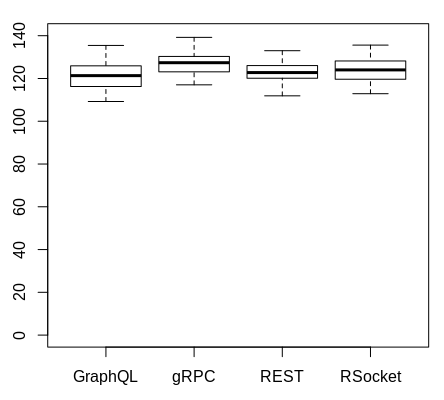
\includegraphics[scale=0.7]{thesis_svava/images/stagger1new.png}}
    \caption{Test case 1: Response times (\textit{ms}) of fetching single delivery.}
    \label{fig:stagger_1}
\end{figure}

\section{Test case 2.A.}
Figure \ref{fig:stagger_2a} shows the results of test case 2.A., fetching a collection of trips, deliveries and users in a single (ad-hoc) request. GraphQL and gRPC show a similar performance with median response times of 182.59 and 179.64 \textit{ms}, respectively. RSocket is slightly slower with 217.69 \textit{ms} response time, and REST comes in last with a median response time of 315.26 \textit{ms}. All four services required a single request to retrieve all data.

While the performances for RSocket, gRPC and GraphQL are similar here, these results show that even if a custom ad-hoc HTTP endpoint is used in an otherwise RESTful service, the performance can still not keep up with the other protocols.

\begin{figure}[ht!]
    \centerline{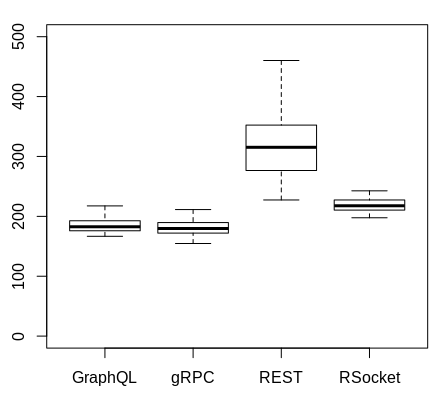
\includegraphics[scale=0.7]{thesis_svava/images/stagger2anew.png}}
    \caption{Test case 2.A.: Response times (\textit{ms}) of fetching trips, deliveries and users in a single request.}
    \label{fig:stagger_2a}
\end{figure}

\section{Test case 2.B.}
Figure \ref{fig:stagger_2b} shows the results of test case 2.B., fetching the same set of objects as 2.A. but in separate requests per resource type for REST, RSocket and gRPC. The result-set for GraphQL here is the same as in Figure \ref{fig:stagger_2a}. GraphQL is now fastest with the median response time of 182.59 \textit{ms}. Next is RSocket, with a 341.59 \textit{ms} response time followed closely by gRPC with 406.99 \textit{ms}. Finally, REST is again the slowest with a median response time of 482.42 \textit{ms}. GraphQL again required only one request, while the other three required in total 30 requests each.

This test case showcases especially well how the GraphQL feature of fetching multiple connected resources in one request improves performance. Furthermore, the performance of gRPC and RSocket is better than for REST, most likely due to the connection reuse feature that both offer.

\begin{figure}[ht!]
    \centerline{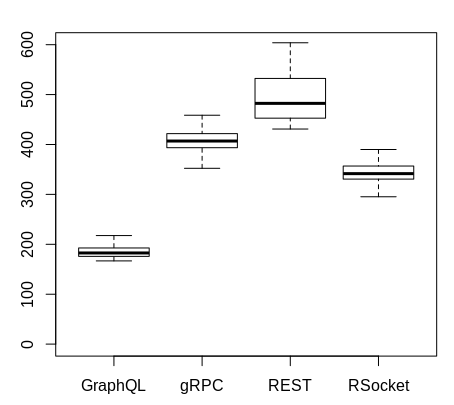
\includegraphics[scale=0.7]{thesis_svava/images/stagger2bnew.png}}
    \caption{Test case 2.B.: Response times (\textit{ms}) of fetching trips, deliveries and users in multiple requests (except GraphQL).}
    \label{fig:stagger_2b}
\end{figure}

\section{Test case 3.A.}
Figure \ref{fig:stagger_3a} shows the results of fetching three different resources in one request each, in parallel. The results are again similar (although not as close as in test case 1) for all four services. GraphQL has a median response time of 130.46 \textit{ms}, gRPC has 142.62 \textit{ms}, REST has 128.65 \textit{ms} and RSocket has 125.26 \textit{ms}.

\begin{figure}[ht!]
    \centerline{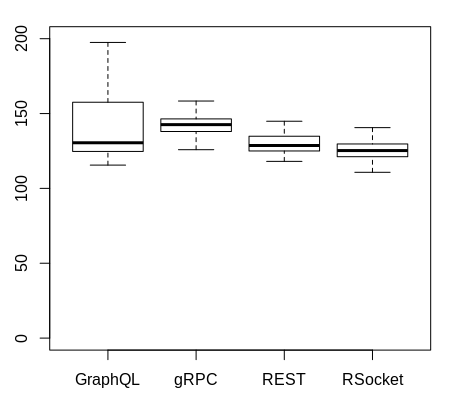
\includegraphics[scale=0.7]{thesis_svava/images/stagger3anew.png}}
    \caption{Test case 3.A.: Response times (\textit{ms}) of fetching a user, a distribution center and delivery IDs in multiple, parallel requests.}
    \label{fig:stagger_3a}
\end{figure}

\section{Test case 3.B.} \label{sec:stagger_3b}
Figure \ref{fig:stagger_3b} shows the results of fetching the same set of objects as 3.A., but in sequence rather than parallel. RSocket now is the fastest with a median response time of 220.19 \textit{ms}. Next is gRPC with a median response time of 294.07 \textit{ms}. Finally, GraphQL and REST have similar results, with median response times of 360.70 and 363.09 \textit{ms}, respectively.

The reason the connection reuse doesn't impact the performance as much in the parallel test case can be explained by the fact that when the three requests are performed in parallel, they are all being handled by the same connection, which could be putting an extra load on that connection. The load thus could be counteracting the benefit provided by not having to re-establish the connection. However, when performed in sequence, the connection only handles one request at a time, so the connection reuse benefit can be enjoyed.

\begin{figure}[ht!]
    \centerline{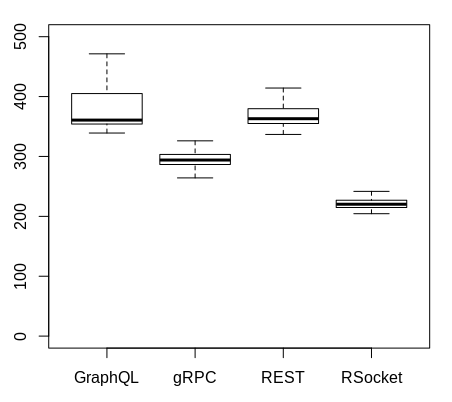
\includegraphics[scale=0.7]{thesis_svava/images/stagger3bnew.png}}
    \caption{Test case 3.B.: Response times (\textit{ms}) of fetching a user, a distribution center and delivery IDs in multiple, sequential requests.}
    \label{fig:stagger_3b}
\end{figure}

The results of these five test cases can be seen in table \ref{tab:results}

\begin{table}
\centering
\label{tab:results}
\begin{tabular}{l|l|l|l|l}
             & GraphQL & gRPC   & REST   & RSocket  \\ 
\hline
Test case 1  & 121.31  & 127.36 & 122.77 & 124.00   \\ 
\hline
Test case 2.A. & 182.59  & 179.64 & 315.26 & 217.69   \\ 
\hline
Test case 2.B. & 182.59  & 406.99 & 482.42 & 341.59   \\ 
\hline
Test case 3.A. & 130.46  & 142.62 & 128.65 & 125.26   \\ 
\hline
Test case 3.B. & 360.70  & 294.07 & 363.09 & 220.19  
\end{tabular}
\caption{Median response time in ms of the five test cases.}
\end{table}

\section{Extra test case - connection reuse}
\begin{figure}
    \centerline{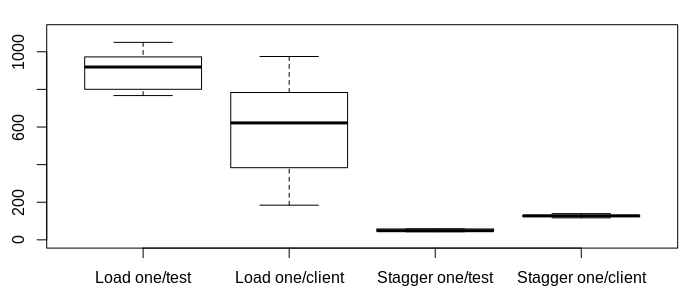
\includegraphics[scale=0.6]{thesis_svava/images/grpcconnections.png}}
    \caption{Response times (\textit{ms}) of gRPC fetching a single delivery.}
    \label{fig:conn_reuse_g}
\end{figure}
\begin{figure}
    \centerline{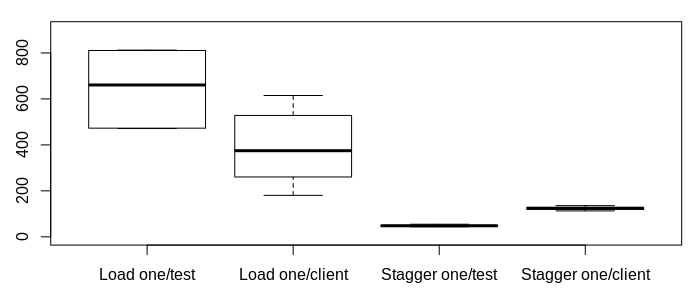
\includegraphics[scale=0.6]{thesis_svava/images/rsocketconnections.png}}
    \caption{Response times (\textit{ms}) of RSocket fetching a single delivery..}
    \label{fig:conn_reuse_r}
\end{figure}
To further illustrate the effect discussed in section \ref{sec:stagger_3b}, two extra tests were performed on RSocket and gRPC: using the same connection for all 100 iterations. Test case 1 was chosen for this. The results obtained previously were compared with a test where all 100 iterations were set off in parallel. The results for each service can be seen in Figures \ref{fig:conn_reuse_r} and \ref{fig:conn_reuse_g}. In both plots, "stagger" refers to the sequential test run with a 0.5 s delay between iterations while "load" refers to the test wherein all iterations are run concurrently.

For both services, we can see that in the staggered mode, the performance is better when using one connection for all 100 iterations since the connection has a chance to "cool down" between requests. However, when running all 100 iterations concurrently, the performance is much better when a new connection is established for each iteration. Here, the performance degradation induced by overloading the single connection far outweighs the benefits of not having to re-establish the connection.

This indicates that for use cases where a single client has to issue a great number of requests to the same server in a short time frame, it may in fact be better to spread the load over multiple connections rather than to reuse the same one.